\chapter{Programación dinámica}

\index{programación dinámica}

\key{Programación dinámica}
es una técnica que combina la corrección
de la búsqueda completa y la eficiencia
de los algoritmos voraces.
La programación dinámica se puede aplicar si el
problema se puede dividir en subproblemas superpuestos
que se pueden resolver independientemente.

Hay dos usos para la programación dinámica:

\begin{itemize}
\item
\key{Encontrar una solución óptima}:
Queremos encontrar una solución que sea
lo más grande o lo más pequeña posible.
\item
\key{Contar el número de soluciones}:
Queremos calcular el número total de
soluciones posibles.
\end{itemize}

Primero veremos cómo la programación dinámica puede
usarse para encontrar una solución óptima,
y luego usaremos la misma idea para
contar las soluciones.

Comprender la programación dinámica es un hito
en la carrera de todo programador competitivo.
Si bien la idea básica es simple,
el desafío es cómo aplicar
la programación dinámica a diferentes problemas.
Este capítulo presenta un conjunto de problemas clásicos
que son un buen punto de partida.

\section{Problema de la moneda}

Primero nos centramos en un problema que ya
hemos visto en el Capítulo 6:
Dado un conjunto de valores de monedas $\texttt{coins} = \{c_1,c_2,\ldots,c_k\}$
y una suma objetivo de dinero $n$, nuestra tarea es
formar la suma $n$ usando la menor cantidad de monedas posible.

En el Capítulo 6, resolvimos el problema usando un
algoritmo voraz que siempre elige la más grande
moneda posible.
El algoritmo voraz funciona, por ejemplo,
cuando las monedas son las monedas de euro,
pero en el caso general el algoritmo voraz
no produce necesariamente una solución óptima.

Ahora es el momento de resolver el problema de manera eficiente
usando programación dinámica, para que el algoritmo
funcione para cualquier conjunto de monedas.
El algoritmo de programación dinámica
se basa en una función recursiva
que recorre todas las posibilidades de cómo
formar la suma, como un algoritmo de fuerza bruta.
Sin embargo, la programación dinámica
algoritmo es eficiente porque
utiliza \emph{memorización} y
calcula la respuesta a cada subproblema solo una vez.

\subsubsection{Formulación recursiva}

La idea en la programación dinámica es
formular el problema de forma recursiva para que
la solución al problema se pueda
calcular a partir de soluciones a problemas más pequeños.
En el problema de la moneda, un problema recursivo natural
es el siguiente:
¿cuál es el menor número de monedas
requerido para formar una suma $x$?

Sea $\texttt{solve}(x)$
denotar el mínimo
número de monedas requeridas para una suma $x$.
Los valores de la función dependen de los
valores de las monedas.
Por ejemplo, si $\texttt{coins} = \{1,3,4\}$,
los primeros valores de la función son los siguientes:

\[
\begin{array}{lcl}
\texttt{solve}(0) & = & 0 \\
\texttt{solve}(1) & = & 1 \\
\texttt{solve}(2) & = & 2 \\
\texttt{solve}(3) & = & 1 \\
\texttt{solve}(4) & = & 1 \\
\texttt{solve}(5) & = & 2 \\
\texttt{solve}(6) & = & 2 \\
\texttt{solve}(7) & = & 2 \\
\texttt{solve}(8) & = & 2 \\
\texttt{solve}(9) & = & 3 \\
\texttt{solve}(10) & = & 3 \\
\end{array}
\]

Por ejemplo, $\texttt{solve}(10)=3$,
porque se necesitan al menos 3 monedas
para formar la suma 10.
La solución óptima es $3+3+4=10$.

La propiedad esencial de $\texttt{solve}$ es
que sus valores se pueden
calcular recursivamente a partir de sus valores más pequeños.
La idea es centrarse en la \emph{primera}
moneda que elegimos para la suma.
Por ejemplo, en el escenario anterior,
la primera moneda puede ser 1, 3 o 4.
Si primero elegimos la moneda 1,
la tarea restante es formar la suma 9
usando el mínimo número de monedas,
que es un subproblema del problema original.
Por supuesto, lo mismo se aplica a las monedas 3 y 4.
Por lo tanto, podemos usar la siguiente fórmula recursiva
para calcular el mínimo número de monedas:
\begin{equation*}
\begin{split}
\texttt{solve}(x) = \min( & \texttt{solve}(x-1)+1, \\
                           & \texttt{solve}(x-3)+1, \\
                           & \texttt{solve}(x-4)+1).
\end{split}
\end{equation*}
El caso base de la recursión es $\texttt{solve}(0)=0$,
porque no se necesitan monedas para formar una suma vacía.
Por ejemplo,
\[ \texttt{solve}(10) = \texttt{solve}(7)+1 = \texttt{solve}(4)+2 = \texttt{solve}(0)+3 = 3.\]

Ahora estamos listos para dar una función recursiva general
que calcula el mínimo número de
monedas necesarias para formar una suma $x$:
\begin{equation*}
    \texttt{solve}(x) = \begin{cases}
               \infty               & x < 0\\
               0               & x = 0\\
               \min_{c \in \texttt{coins}} \texttt{solve}(x-c)+1 & x > 0 \\
           \end{cases}
\end{equation*}

Primero, si $x<0$, el valor es $\infty$,
porque es imposible formar una suma negativa
de dinero.
Luego, si $x=0$, el valor es $0$,
porque no se necesitan monedas para formar una suma vacía.
Finalmente, si $x>0$, la variable $c$ pasa por
todas las posibilidades de cómo elegir la primera moneda
de la suma.

Una vez que se ha encontrado una función recursiva que resuelve el problema,
podemos implementar directamente una solución en C++
(la constante \texttt{INF} denota infinito):
\begin{lstlisting}
int solve(int x) {
    if (x < 0) return INF;
    if (x == 0) return 0;
    int best = INF;
    for (auto c : coins) {
        best = min(best, solve(x-c)+1);
    }
    return best;
}
\end{lstlisting}

Aún así, esta función no es eficiente,
porque puede haber un número exponencial de formas
de construir la suma.
Sin embargo, a continuación veremos cómo hacer que la
función sea eficiente utilizando una técnica llamada memorización.

\subsubsection{Usando memorización}

\index{memorización}

La idea de la programación dinámica es usar
\key{memorización} para calcular eficientemente
los valores de una función recursiva.
Esto significa que los valores de la función
se almacenan en una matriz después de calcularlos.
Para cada parámetro, el valor de la función
se calcula recursivamente solo una vez, y después de esto,
el valor se puede recuperar directamente de la matriz.

En este problema, usamos matrices
\begin{lstlisting}
bool ready[N];
int value[N];
\end{lstlisting}

donde $\texttt{ready}[x]$ indica
si el valor de $\texttt{solve}(x)$ ya se ha calculado,
y si es así, $\texttt{value}[x]$
contiene este valor.
La constante $N$ se ha elegido de modo que
todos los valores necesarios quepan en las matrices.

Ahora la función se puede implementar eficientemente
de la siguiente manera:

\begin{lstlisting}
int solve(int x) {
    if (x < 0) return INF;
    if (x == 0) return 0;
    if (ready[x]) return value[x];
    int best = INF;
    for (auto c : coins) {
        best = min(best, solve(x-c)+1);
    }
    value[x] = best;
    ready[x] = true;
    return best;
}
\end{lstlisting}

La función maneja los casos base
$x<0$ y $x=0$ como antes.
Luego, la función verifica desde
$\texttt{ready}[x]$ si
$\texttt{solve}(x)$ ya se ha almacenado
en $\texttt{value}[x]$,
y si es así, la función la devuelve directamente.
De lo contrario, la función calcula el valor
de $\texttt{solve}(x)$
recursivamente y lo almacena en $\texttt{value}[x]$.

Esta función funciona eficientemente,
porque la respuesta para cada parámetro $x$
se calcula recursivamente solo una vez.
Una vez que un valor de $\texttt{solve}(x)$ se ha almacenado en $\texttt{value}[x]$,
se puede recuperar eficientemente cada vez que la
función se vuelva a llamar con el parámetro $x$.
La complejidad temporal del algoritmo es $O(nk)$,
donde $n$ es la suma objetivo y $k$ es la cantidad de monedas.

Tenga en cuenta que también podemos \emph{iterativamente}
construir la matriz \texttt{value} utilizando
un bucle que simplemente calcula todos los valores
de $\texttt{solve}$ para los parámetros $0 \ldots n$:
\begin{lstlisting}
value[0] = 0;
for (int x = 1; x <= n; x++) {
    value[x] = INF;
    for (auto c : coins) {
        if (x-c >= 0) {
            value[x] = min(value[x], value[x-c]+1);
        }
    }
}
\end{lstlisting}

De hecho, la mayoría de los programadores competitivos prefieren esta
implementación, porque es más corta y tiene
factores constantes más bajos.
De ahora en adelante, también usamos implementaciones iterativas
en nuestros ejemplos.
Aún así, a menudo es más fácil pensar en
soluciones de programación dinámica
en términos de funciones recursivas.


\subsubsection{Construyendo una solución}

A veces se nos pide que encontremos el valor
de una solución óptima y que demos
un ejemplo de cómo se puede construir una solución de este tipo.
En el problema de la moneda, por ejemplo,
podemos declarar otra matriz
que indique para
cada suma de dinero la primera moneda
en una solución óptima:
\begin{lstlisting}
int first[N];
\end{lstlisting}
Luego, podemos modificar el algoritmo de la siguiente manera:
\begin{lstlisting}
value[0] = 0;
for (int x = 1; x <= n; x++) {
    value[x] = INF;
    for (auto c : coins) {
        if (x-c >= 0 && value[x-c]+1 < value[x]) {
            value[x] = value[x-c]+1;
            first[x] = c;
        }
    }
}
\end{lstlisting}
Después de esto, el siguiente código se puede usar para
imprimir las monedas que aparecen en una solución óptima para
la suma $n$:
\begin{lstlisting}
while (n > 0) {
    cout << first[n] << "\n";
    n -= first[n];
}
\end{lstlisting}

\subsubsection{Contando el número de soluciones}

Consideremos ahora otra versión
del problema de la moneda donde nuestra tarea es
calcular el número total de formas
de producir una suma $x$ usando las monedas.
Por ejemplo, si $\texttt{coins}=\{1,3,4\}$ y
$x=5$, hay un total de 6 formas:

\begin{multicols}{2}
\begin{itemize}
\item $1+1+1+1+1$
\item $1+1+3$
\item $1+3+1$
\item $3+1+1$
\item $1+4$
\item $4+1$
\end{itemize}
\end{multicols}

Nuevamente, podemos resolver el problema recursivamente.
Sea $\texttt{solve}(x)$ denotar el número de formas
en que podemos formar la suma $x$.
Por ejemplo, si $\texttt{coins}=\{1,3,4\}$,
entonces $\texttt{solve}(5)=6$ y la fórmula recursiva es
\begin{equation*}
\begin{split}
\texttt{solve}(x) = & \texttt{solve}(x-1) + \\
                    & \texttt{solve}(x-3) + \\
                    & \texttt{solve}(x-4)  .
\end{split}
\end{equation*}
Entonces, la función recursiva general es la siguiente:
\begin{equation*}
    \texttt{solve}(x) = \begin{cases}
               0               & x < 0\\
               1               & x = 0\\
               \sum_{c \in \texttt{coins}} \texttt{solve}(x-c) & x > 0 \\
           \end{cases}
\end{equation*}

Si $x<0$, el valor es 0, porque no hay soluciones.
Si $x=0$, el valor es 1, porque solo hay una forma
de formar una suma vacía.
De lo contrario, calculamos la suma de todos los valores
de la forma $\texttt{solve}(x-c)$ donde $c$ está en \texttt{coins}.

El siguiente código construye un arreglo
$\texttt{count}$ tal que
$\texttt{count}[x]$ es igual
al valor de $\texttt{solve}(x)$
para $0 \le x \le n$:

\begin{lstlisting}
count[0] = 1;
for (int x = 1; x <= n; x++) {
    for (auto c : coins) {
        if (x-c >= 0) {
            count[x] += count[x-c];
        }
    }
}
\end{lstlisting}

A menudo, el número de soluciones es tan grande
que no es necesario calcular el número exacto,
pero es suficiente dar la respuesta módulo $m$
donde, por ejemplo, $m=10^9+7$.
Esto se puede hacer cambiando el código para que
todos los cálculos se realicen módulo $m$.
En el código anterior, basta con agregar la línea
\begin{lstlisting}
        count[x] %= m;
\end{lstlisting}
después de la línea
\begin{lstlisting}
        count[x] += count[x-c];
\end{lstlisting}

Ahora hemos discutido todas las ideas básicas
de la programación dinámica.
Dado que la programación dinámica se puede utilizar
en muchas situaciones diferentes,
ahora veremos un conjunto de problemas
que muestran más ejemplos sobre las
posibilidades de la programación dinámica.

\section{Subsecuencia creciente más larga}

\index{subsecuencia creciente más larga}

Nuestro primer problema es encontrar la
\key{subsecuencia creciente más larga}
en un arreglo de $n$ elementos.
Esta es una secuencia de longitud máxima
de elementos del arreglo
que va de izquierda a derecha,
y cada elemento de la secuencia es mayor
que el elemento anterior.
Por ejemplo, en el arreglo

\begin{center}
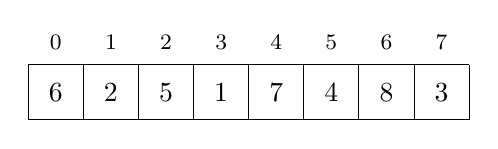
\begin{tikzpicture}[scale=0.7]
\draw (0,0) grid (8,1);
\node at (0.5,0.5) {$6$};
\node at (1.5,0.5) {$2$};
\node at (2.5,0.5) {$5$};
\node at (3.5,0.5) {$1$};
\node at (4.5,0.5) {$7$};
\node at (5.5,0.5) {$4$};
\node at (6.5,0.5) {$8$};
\node at (7.5,0.5) {$3$};

\footnotesize
\node at (0.5,1.4) {$0$};
\node at (1.5,1.4) {$1$};
\node at (2.5,1.4) {$2$};
\node at (3.5,1.4) {$3$};
\node at (4.5,1.4) {$4$};
\node at (5.5,1.4) {$5$};
\node at (6.5,1.4) {$6$};
\node at (7.5,1.4) {$7$};
\end{tikzpicture}
\end{center}
la subsecuencia creciente más larga
contiene 4 elementos:
\begin{center}
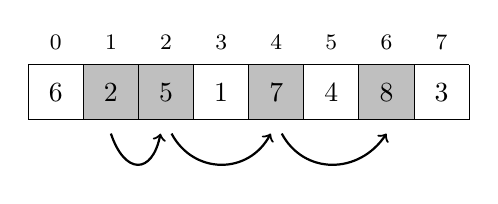
\begin{tikzpicture}[scale=0.7]
\fill[color=lightgray] (1,0) rectangle (2,1);
\fill[color=lightgray] (2,0) rectangle (3,1);
\fill[color=lightgray] (4,0) rectangle (5,1);
\fill[color=lightgray] (6,0) rectangle (7,1);
\draw (0,0) grid (8,1);
\node at (0.5,0.5) {$6$};
\node at (1.5,0.5) {$2$};
\node at (2.5,0.5) {$5$};
\node at (3.5,0.5) {$1$};
\node at (4.5,0.5) {$7$};
\node at (5.5,0.5) {$4$};
\node at (6.5,0.5) {$8$};
\node at (7.5,0.5) {$3$};

\draw[thick,->] (1.5,-0.25) .. controls (1.75,-1.00) and (2.25,-1.00) .. (2.4,-0.25);
\draw[thick,->] (2.6,-0.25) .. controls (3.0,-1.00) and (4.0,-1.00) .. (4.4,-0.25);
\draw[thick,->] (4.6,-0.25) .. controls (5.0,-1.00) and (6.0,-1.00) .. (6.5,-0.25);

\footnotesize
\node at (0.5,1.4) {$0$};
\node at (1.5,1.4) {$1$};
\node at (2.5,1.4) {$2$};
\node at (3.5,1.4) {$3$};
\node at (4.5,1.4) {$4$};
\node at (5.5,1.4) {$5$};
\node at (6.5,1.4) {$6$};
\node at (7.5,1.4) {$7$};
\end{tikzpicture}
\end{center}

Sea $\texttt{length}(k)$ denotar
la longitud de la
subsecuencia creciente más larga
que termina en la posición $k$.
Así, si calculamos todos los valores de
$\texttt{length}(k)$ donde $0 \le k \le n-1$,
descubriremos la longitud de la
subsecuencia creciente más larga.
Por ejemplo, los valores de la función
para el arreglo anterior son los siguientes:
\[
\begin{array}{lcl}
\texttt{length}(0) & = & 1 \\
\texttt{length}(1) & = & 1 \\
\texttt{length}(2) & = & 2 \\
\texttt{length}(3) & = & 1 \\
\texttt{length}(4) & = & 3 \\
\texttt{length}(5) & = & 2 \\
\texttt{length}(6) & = & 4 \\
\texttt{length}(7) & = & 2 \\
\end{array}
\]

Por ejemplo, $\texttt{length}(6)=4$,
porque la subsecuencia creciente más larga
que termina en la posición 6 consta de 4 elementos.

Para calcular un valor de $\texttt{length}(k)$,
debemos encontrar una posición $i<k$
para la cual $\texttt{array}[i]<\texttt{array}[k]$
y $\texttt{length}(i)$ sea lo más grande posible.
Entonces sabemos que
$\texttt{length}(k)=\texttt{length}(i)+1$,
porque esta es una forma óptima de agregar
$\texttt{array}[k]$ a una subsecuencia.
Sin embargo, si no existe tal posición $i$,
entonces $\texttt{length}(k)=1$,
lo que significa que la subsecuencia solo contiene
$\texttt{array}[k]$.

Dado que todos los valores de la función se pueden calcular
a partir de sus valores más pequeños,
podemos usar la programación dinámica.
En el siguiente código, los valores
de la función se almacenarán en un arreglo
$\texttt{length}$.
\begin{lstlisting}
for (int k = 0; k < n; k++) {
    length[k] = 1;
    for (int i = 0; i < k; i++) {
        if (array[i] < array[k]) {
            length[k] = max(length[k],length[i]+1);
        }
    }
}
\end{lstlisting}

Este código funciona en tiempo $O(n^2)$,
porque consiste en dos bucles anidados.
Sin embargo, también es posible implementar
el cálculo de programación dinámica
de forma más eficiente en tiempo $O(n \log n)$.
¿Puedes encontrar una manera de hacer esto?

\section{Caminos en una cuadrícula}

Nuestro próximo problema es encontrar un camino
desde la esquina superior izquierda hasta
la esquina inferior derecha
de una cuadrícula de $n \times n$, de modo que
solo nos movamos hacia abajo y hacia la derecha.
Cada cuadrado contiene un entero positivo,
y el camino debe construirse de modo que
la suma de los valores a lo largo
del camino sea lo más grande posible.

La siguiente imagen muestra un camino óptimo
en una cuadrícula:
\begin{center}
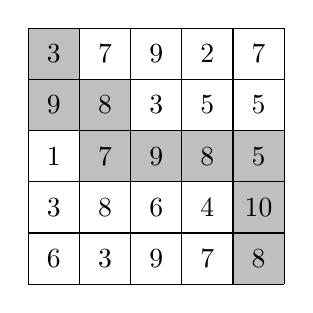
\begin{tikzpicture}[scale=.65]
  \begin{scope}
    \fill [color=lightgray] (0, 9) rectangle (1, 8);
    \fill [color=lightgray] (0, 8) rectangle (1, 7);
    \fill [color=lightgray] (1, 8) rectangle (2, 7);
    \fill [color=lightgray] (1, 7) rectangle (2, 6);
    \fill [color=lightgray] (2, 7) rectangle (3, 6);
    \fill [color=lightgray] (3, 7) rectangle (4, 6);
    \fill [color=lightgray] (4, 7) rectangle (5, 6);
    \fill [color=lightgray] (4, 6) rectangle (5, 5);
    \fill [color=lightgray] (4, 5) rectangle (5, 4);
    \draw (0, 4) grid (5, 9);
    \node at (0.5,8.5) {3};
    \node at (1.5,8.5) {7};
    \node at (2.5,8.5) {9};
    \node at (3.5,8.5) {2};
    \node at (4.5,8.5) {7};
    \node at (0.5,7.5) {9};
    \node at (1.5,7.5) {8};
    \node at (2.5,7.5) {3};
    \node at (3.5,7.5) {5};
    \node at (4.5,7.5) {5};
    \node at (0.5,6.5) {1};
    \node at (1.5,6.5) {7};
    \node at (2.5,6.5) {9};
    \node at (3.5,6.5) {8};
    \node at (4.5,6.5) {5};
    \node at (0.5,5.5) {3};
    \node at (1.5,5.5) {8};
    \node at (2.5,5.5) {6};
    \node at (3.5,5.5) {4};
    \node at (4.5,5.5) {10};
    \node at (0.5,4.5) {6};
    \node at (1.5,4.5) {3};
    \node at (2.5,4.5) {9};
    \node at (3.5,4.5) {7};
    \node at (4.5,4.5) {8};
  \end{scope}
\end{tikzpicture}
\end{center}
La suma de los valores en el camino es 67,
y esta es la suma más grande posible en un camino
desde la
esquina superior izquierda hasta la esquina inferior derecha.

Asuma que las filas y columnas de la
cuadrícula están numeradas de 1 a $n$,
y $\texttt{value}[y][x]$ es igual al valor
del cuadrado $(y,x)$.
Sea $\texttt{sum}(y,x)$ la suma máxima
en un camino desde la esquina superior izquierda
hasta el cuadrado $(y,x)$.
Ahora $\texttt{sum}(n,n)$ nos dice
la suma máxima
desde la esquina superior izquierda hasta
la esquina inferior derecha.
Por ejemplo, en la cuadrícula de arriba,
$\texttt{sum}(5,5)=67$.

Podemos calcular recursivamente las sumas
de la siguiente manera:
\[ \texttt{sum}(y,x) = \max(\texttt{sum}(y,x-1),\texttt{sum}(y-1,x))+\texttt{value}[y][x]\]


La fórmula recursiva se basa en la observación
de que un camino que termina en el cuadrado $(y,x)$
puede venir ya sea del cuadrado $(y,x-1)$
o del cuadrado $(y-1,x)$:
\begin{center}
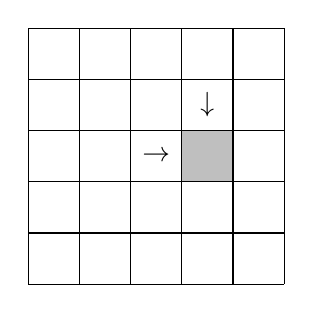
\begin{tikzpicture}[scale=.65]
  \begin{scope}
    \fill [color=lightgray] (3, 7) rectangle (4, 6);
    \draw (0, 4) grid (5, 9);
    
    \node at (2.5,6.5) {$\rightarrow$};
    \node at (3.5,7.5) {$\downarrow$};
    
  \end{scope}
\end{tikzpicture}
\end{center}

Por lo tanto, seleccionamos la dirección que maximiza
la suma.
Asumamos que $\texttt{sum}(y,x)=0$
si $y=0$ o $x=0$ (porque no existen tales caminos),
por lo que la fórmula recursiva también funciona cuando $y=1$ o $x=1$.

Dado que la función \texttt{sum} tiene dos parámetros,
la matriz de programación dinámica también tiene dos dimensiones.
Por ejemplo, podemos usar una matriz
\begin{lstlisting}
int sum[N][N];
\end{lstlisting}
y calcular las sumas de la siguiente manera:
\begin{lstlisting}
for (int y = 1; y <= n; y++) {
    for (int x = 1; x <= n; x++) {
        sum[y][x] = max(sum[y][x-1],sum[y-1][x])+value[y][x];
    }
}
\end{lstlisting}
La complejidad temporal del algoritmo es $O(n^2)$.

\section{Problemas de la mochila}

\index{mochila}

El término \key{mochila} se refiere a problemas donde
se da un conjunto de objetos, y 
se deben encontrar subconjuntos con algunas propiedades.
Los problemas de la mochila a menudo se pueden resolver
utilizando programación dinámica.

En esta sección, nos centraremos en el siguiente
problema: Dado una lista de pesos
$[w_1,w_2,\ldots,w_n]$,
determinar todas
las sumas que se pueden construir utilizando los pesos.
Por ejemplo, si los pesos son
$[1,3,3,5]$, las siguientes sumas son posibles:

\begin{center}
\begin{tabular}{rrrrrrrrrrrrr}
 0 & 1 & 2 & 3 & 4 & 5 & 6 & 7 & 8 & 9 & 10 & 11 & 12 \\
\hline
 X & X & & X & X & X & X & X & X & X & & X & X \\
\end{tabular}
\end{center}

En este caso, todas las sumas entre $0 \ldots 12$
son posibles, excepto 2 y 10.
Por ejemplo, la suma 7 es posible porque
podemos seleccionar los pesos $[1,3,3]$.


Para resolver el problema, nos centramos en subproblemas
donde solo usamos los primeros $k$ pesos
para construir sumas.
Sea $\texttt{possible}(x,k)=\textrm{true}$ si
podemos construir una suma $x$
usando los primeros $k$ pesos,
y de lo contrario $\texttt{possible}(x,k)=\textrm{false}$.
Los valores de la función se pueden calcular recursivamente
como sigue:
\[ \texttt{possible}(x,k) = \texttt{possible}(x-w_k,k-1) \lor \texttt{possible}(x,k-1) \]
La fórmula se basa en el hecho de que podemos
usar o no usar el peso $w_k$ en la suma.
Si usamos $w_k$, la tarea restante es
formar la suma $x-w_k$ usando los primeros $k-1$ pesos,
y si no usamos $w_k$,
la tarea restante es formar la suma $x$
usando los primeros $k-1$ pesos.
Como casos base,
\begin{equation*}
    \texttt{possible}(x,0) = \begin{cases}
               \textrm{true}    & x = 0\\
               \textrm{false}   & x \neq 0 \\
           \end{cases}
\end{equation*}
porque si no se usan pesos,
solo podemos formar la suma 0.

La siguiente tabla muestra todos los valores de la función
para los pesos $[1,3,3,5]$ (el símbolo ''X''
indica los valores verdaderos):

\begin{center}
\begin{tabular}{r|rrrrrrrrrrrrr}
$k \backslash x$ & 0 & 1 & 2 & 3 & 4 & 5 & 6 & 7 & 8 & 9 & 10 & 11 & 12 \\
\hline
 0 & X & \\
 1 & X & X \\
 2 & X & X & & X & X \\
 3 & X & X & & X & X & & X & X \\
 4 & X & X & & X & X & X & X & X & X & X & & X & X \\
\end{tabular}
\end{center}

Después de calcular esos valores, $\texttt{possible}(x,n)$
nos dice si podemos construir una
suma $x$ usando \emph{todos} los pesos.

Sea $W$ la suma total de los pesos.
La siguiente solución de programación dinámica de tiempo $O(nW)$
corresponde a la función recursiva:
\begin{lstlisting}
possible[0][0] = true;
for (int k = 1; k <= n; k++) {
    for (int x = 0; x <= W; x++) {
        if (x-w[k] >= 0) possible[x][k] |= possible[x-w[k]][k-1];
        possible[x][k] |= possible[x][k-1];
    }
}
\end{lstlisting}

Sin embargo, aquí hay una mejor implementación que solo usa
una matriz unidimensional $\texttt{possible}[x]$
que indica si podemos construir un subconjunto con suma $x$.
El truco es actualizar la matriz de derecha a izquierda para
cada nuevo peso:
\begin{lstlisting}
possible[0] = true;
for (int k = 1; k <= n; k++) {
    for (int x = W; x >= 0; x--) {
        if (possible[x]) possible[x+w[k]] = true;
    }
}
\end{lstlisting}

Tenga en cuenta que la idea general presentada aquí se puede utilizar
en muchos problemas de mochila.
Por ejemplo, si se nos dan objetos con pesos y valores,
podemos determinar para cada suma de peso la suma de valor máximo
de un subconjunto.

\section{Distancia de edición}

\index{distancia de edición}
\index{distancia de Levenshtein}

La \key{distancia de edición} o \key{distancia de Levenshtein}\footnote{La distancia
recibe el nombre de V. I. Levenshtein quien la estudió en relación con los códigos binarios \cite{lev66}.}
es el número mínimo de operaciones de edición
necesarias para transformar una cadena
en otra cadena.
Las operaciones de edición permitidas son las siguientes:
\begin{itemize}
\item insertar un carácter (por ejemplo, \texttt{ABC} $\rightarrow$ \texttt{ABCA})
\item eliminar un carácter (por ejemplo, \texttt{ABC} $\rightarrow$ \texttt{AC})
\item modificar un carácter (por ejemplo, \texttt{ABC} $\rightarrow$ \texttt{ADC})
\end{itemize}

Por ejemplo, la distancia de edición entre
\texttt{LOVE} y \texttt{MOVIE} es 2,
porque primero podemos realizar la operación
 \texttt{LOVE} $\rightarrow$ \texttt{MOVE}
(modificar) y luego la operación
\texttt{MOVE} $\rightarrow$ \texttt{MOVIE}
(insertar).
Este es el menor número posible de operaciones,
porque está claro que solo una operación no es suficiente.

Suponga que se nos da una cadena \texttt{x}
de longitud $n$ y una cadena \texttt{y} de longitud $m$,
y queremos calcular la distancia de edición entre
\texttt{x} y \texttt{y}.
Para resolver el problema, definimos una función
$\texttt{distance}(a,b)$ que da la
distancia de edición entre prefijos
$\texttt{x}[0 \ldots a]$ y $\texttt{y}[0 \ldots b]$.
Por lo tanto, usando esta función, la distancia de edición
entre \texttt{x} y \texttt{y} es igual a $\texttt{distance}(n-1,m-1)$.
Podemos calcular los valores de \texttt{distance}
de la siguiente manera:
\begin{equation*}
\begin{split}
\texttt{distance}(a,b) = \min(& \texttt{distance}(a,b-1)+1, \\
                           & \texttt{distance}(a-1,b)+1, \\
                           & \texttt{distance}(a-1,b-1)+\texttt{cost}(a,b)).
\end{split}
\end{equation*}
Aquí $\texttt{cost}(a,b)=0$ si $\texttt{x}[a]=\texttt{y}[b]$,
y de lo contrario $\texttt{cost}(a,b)=1$.
La fórmula considera las siguientes formas de
editar la cadena \texttt{x}:
\begin{itemize}
\item $\texttt{distance}(a,b-1)$: insertar un carácter al final de \texttt{x}
\item $\texttt{distance}(a-1,b)$: eliminar el último carácter de \texttt{x}
\item $\texttt{distance}(a-1,b-1)$: coincidir o modificar el último carácter de \texttt{x}
\end{itemize}
En los dos primeros casos, se necesita una operación de edición
(insertar o eliminar).
En el último caso, si $\texttt{x}[a]=\texttt{y}[b]$,
podemos hacer coincidir los últimos caracteres sin editar,
y de lo contrario se necesita una operación de edición (modificar).

La siguiente tabla muestra los valores de \texttt{distance}
en el caso de ejemplo:
\begin{center}
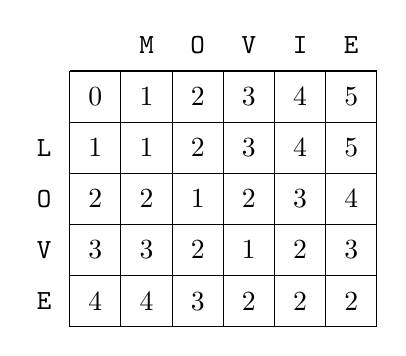
\begin{tikzpicture}[scale=.65]
  \begin{scope}
    %\fill [color=lightgray] (5, -3) rectangle (6, -4);
    \draw (1, -1) grid (7, -6);
    
    \node at (0.5,-2.5) {\texttt{L}};
    \node at (0.5,-3.5) {\texttt{O}};
    \node at (0.5,-4.5) {\texttt{V}};
    \node at (0.5,-5.5) {\texttt{E}};

    \node at (2.5,-0.5) {\texttt{M}};
    \node at (3.5,-0.5) {\texttt{O}};
    \node at (4.5,-0.5) {\texttt{V}};
    \node at (5.5,-0.5) {\texttt{I}};
    \node at (6.5,-0.5) {\texttt{E}};

    \node at (1.5,-1.5) {$0$};
    \node at (1.5,-2.5) {$1$};
    \node at (1.5,-3.5) {$2$};
    \node at (1.5,-4.5) {$3$};
    \node at (1.5,-5.5) {$4$};
    \node at (2.5,-1.5) {$1$};
    \node at (2.5,-2.5) {$1$};
    \node at (2.5,-3.5) {$2$};
    \node at (2.5,-4.5) {$3$};
    \node at (2.5,-5.5) {$4$};
    \node at (3.5,-1.5) {$2$};
    \node at (3.5,-2.5) {$2$};
    \node at (3.5,-3.5) {$1$};
    \node at (3.5,-4.5) {$2$};
    \node at (3.5,-5.5) {$3$};
    \node at (4.5,-1.5) {$3$};
    \node at (4.5,-2.5) {$3$};
    \node at (4.5,-3.5) {$2$};
    \node at (4.5,-4.5) {$1$};
    \node at (4.5,-5.5) {$2$};
    \node at (5.5,-1.5) {$4$};
    \node at (5.5,-2.5) {$4$};
    \node at (5.5,-3.5) {$3$};
    \node at (5.5,-4.5) {$2$};
    \node at (5.5,-5.5) {$2$};
    \node at (6.5,-1.5) {$5$};
    \node at (6.5,-2.5) {$5$};
    \node at (6.5,-3.5) {$4$};
    \node at (6.5,-4.5) {$3$};
    \node at (6.5,-5.5) {$2$};
  \end{scope}
\end{tikzpicture}
\end{center}

La esquina inferior derecha de la tabla
nos dice que la distancia de edición entre
\texttt{LOVE} y \texttt{MOVIE} es 2.
La tabla también muestra cómo construir
la secuencia más corta de operaciones de edición.
En este caso, la ruta es la siguiente:

\begin{center}
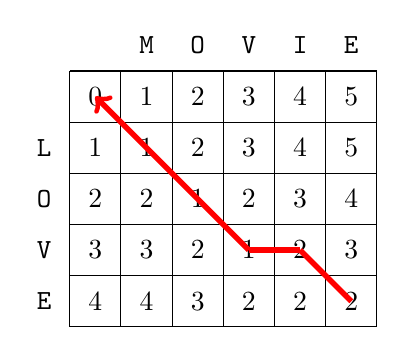
\begin{tikzpicture}[scale=.65]
  \begin{scope}
    \draw (1, -1) grid (7, -6);
    
    \node at (0.5,-2.5) {\texttt{L}};
    \node at (0.5,-3.5) {\texttt{O}};
    \node at (0.5,-4.5) {\texttt{V}};
    \node at (0.5,-5.5) {\texttt{E}};

    \node at (2.5,-0.5) {\texttt{M}};
    \node at (3.5,-0.5) {\texttt{O}};
    \node at (4.5,-0.5) {\texttt{V}};
    \node at (5.5,-0.5) {\texttt{I}};
    \node at (6.5,-0.5) {\texttt{E}};

    \node at (1.5,-1.5) {$0$};
    \node at (1.5,-2.5) {$1$};
    \node at (1.5,-3.5) {$2$};
    \node at (1.5,-4.5) {$3$};
    \node at (1.5,-5.5) {$4$};
    \node at (2.5,-1.5) {$1$};
    \node at (2.5,-2.5) {$1$};
    \node at (2.5,-3.5) {$2$};
    \node at (2.5,-4.5) {$3$};
    \node at (2.5,-5.5) {$4$};
    \node at (3.5,-1.5) {$2$};
    \node at (3.5,-2.5) {$2$};
    \node at (3.5,-3.5) {$1$};
    \node at (3.5,-4.5) {$2$};
    \node at (3.5,-5.5) {$3$};
    \node at (4.5,-1.5) {$3$};
    \node at (4.5,-2.5) {$3$};
    \node at (4.5,-3.5) {$2$};
    \node at (4.5,-4.5) {$1$};
    \node at (4.5,-5.5) {$2$};
    \node at (5.5,-1.5) {$4$};
    \node at (5.5,-2.5) {$4$};
    \node at (5.5,-3.5) {$3$};
    \node at (5.5,-4.5) {$2$};
    \node at (5.5,-5.5) {$2$};
    \node at (6.5,-1.5) {$5$};
    \node at (6.5,-2.5) {$5$};
    \node at (6.5,-3.5) {$4$};
    \node at (6.5,-4.5) {$3$};
    \node at (6.5,-5.5) {$2$};

    \path[draw=red,thick,-,line width=2pt] (6.5,-5.5) -- (5.5,-4.5);
    \path[draw=red,thick,-,line width=2pt] (5.5,-4.5) -- (4.5,-4.5);
    \path[draw=red,thick,->,line width=2pt] (4.5,-4.5) -- (1.5,-1.5);
  \end{scope}
\end{tikzpicture}
\end{center}

Los últimos caracteres de \texttt{LOVE} y \texttt{MOVIE}
son iguales, por lo que la distancia de edición entre ellos
es igual a la distancia de edición entre \texttt{LOV} y \texttt{MOVI}.
Podemos usar una operación de edición para eliminar el
carácter \texttt{I} de \texttt{MOVI}.
Por lo tanto, la distancia de edición es uno mayor que
la distancia de edición entre \texttt{LOV} y \texttt{MOV}, etc.

\section{Contando mosaicos}


A veces, los estados de una solución de programación dinámica
son más complejos que las combinaciones fijas de números.
Como ejemplo,
considere el problema de calcular
el número de maneras distintas de
llenar una cuadrícula de $n \times m$ usando
baldosas de tamaño $1 \times 2$ y $2 \times 1$.
Por ejemplo, una solución válida
para la cuadrícula de $4 \times 7$ es
\begin{center}
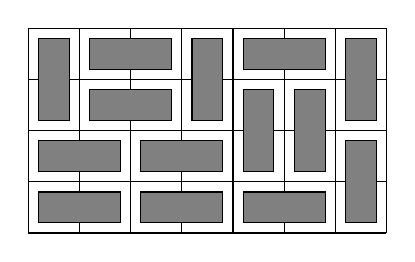
\begin{tikzpicture}[scale=.65]
    \draw (0,0) grid (7,4);
    \draw[fill=gray] (0+0.2,0+0.2) rectangle (2-0.2,1-0.2);
    \draw[fill=gray] (2+0.2,0+0.2) rectangle (4-0.2,1-0.2);
    \draw[fill=gray] (4+0.2,0+0.2) rectangle (6-0.2,1-0.2);
    \draw[fill=gray] (0+0.2,1+0.2) rectangle (2-0.2,2-0.2);
    \draw[fill=gray] (2+0.2,1+0.2) rectangle (4-0.2,2-0.2);
    \draw[fill=gray] (1+0.2,2+0.2) rectangle (3-0.2,3-0.2);
    \draw[fill=gray] (1+0.2,3+0.2) rectangle (3-0.2,4-0.2);
    \draw[fill=gray] (4+0.2,3+0.2) rectangle (6-0.2,4-0.2);

    \draw[fill=gray] (0+0.2,2+0.2) rectangle (1-0.2,4-0.2);
    \draw[fill=gray] (3+0.2,2+0.2) rectangle (4-0.2,4-0.2);
    \draw[fill=gray] (6+0.2,2+0.2) rectangle (7-0.2,4-0.2);
    \draw[fill=gray] (4+0.2,1+0.2) rectangle (5-0.2,3-0.2);
    \draw[fill=gray] (5+0.2,1+0.2) rectangle (6-0.2,3-0.2);
    \draw[fill=gray] (6+0.2,0+0.2) rectangle (7-0.2,2-0.2);

\end{tikzpicture}
\end{center}
y el número total de soluciones es 781.

El problema se puede resolver usando programación dinámica
recorriendo la cuadrícula fila por fila.
Cada fila en una solución se puede representar como una
cadena que contiene $m$ caracteres del conjunto
$\{\sqcap, \sqcup, \sqsubset, \sqsupset \}$.
Por ejemplo, la solución anterior consta de cuatro filas
que corresponden a las siguientes cadenas:
\begin{itemize}
\item
$\sqcap \sqsubset \sqsupset \sqcap \sqsubset \sqsupset \sqcap$
\item
$\sqcup \sqsubset \sqsupset \sqcup \sqcap \sqcap \sqcup$
\item
$\sqsubset \sqsupset \sqsubset \sqsupset \sqcup \sqcup \sqcap$ 
\item
$\sqsubset \sqsupset \sqsubset \sqsupset \sqsubset \sqsupset \sqcup$
\end{itemize}

Sea $\texttt{count}(k,x)$ el número de maneras de
construir una solución para las filas $1 \ldots k$
de la cuadrícula tal que la cadena $x$ corresponde a la fila $k$.
Es posible usar programación dinámica aquí,
porque el estado de una fila está limitado
solo por el estado de la fila anterior.

Una solución es válida si la fila $1$ no contiene
el carácter $\sqcup$,
la fila $n$ no contiene el carácter $\sqcap$,
y todas las filas consecutivas son \emph{compatibles}.
Por ejemplo, las filas
$\sqcup \sqsubset \sqsupset \sqcup \sqcap \sqcap \sqcup$ y
$\sqsubset \sqsupset \sqsubset \sqsupset \sqcup \sqcup \sqcap$ 
son compatibles, mientras que las filas
$\sqcap \sqsubset \sqsupset \sqcap \sqsubset \sqsupset \sqcap$ y
$\sqsubset \sqsupset \sqsubset \sqsupset \sqsubset \sqsupset \sqcup$
no son compatibles.

Dado que una fila consta de $m$ caracteres y hay
cuatro opciones para cada carácter, el número de distintas
filas es como máximo $4^m$.
Por lo tanto, la complejidad temporal de la solución es
$O(n 4^{2m})$ porque podemos recorrer las
$O(4^m)$ posibles estados para cada fila,
y para cada estado, hay $O(4^m)$
posibles estados para la fila anterior.
En la práctica, es una buena idea rotar la cuadrícula
para que el lado más corto tenga longitud $m$,
porque el factor $4^{2m}$ domina la complejidad temporal.

Es posible hacer que la solución sea más eficiente
usando una representación más compacta para las filas.
Resulta que es suficiente saber cuáles
columnas de la fila anterior contienen el cuadrado superior
de una baldosa vertical.
Por lo tanto, podemos representar una fila usando solo caracteres
$\sqcap$ y $\Box$, donde $\Box$ es una combinación
de caracteres
$\sqcup$, $\sqsubset$ y $\sqsupset$.
Usando esta representación, solo hay
$2^m$ filas distintas y la complejidad temporal es
$O(n 2^{2m})$.

Como nota final, también existe una sorprendente fórmula directa
para calcular el número de teselaciones\footnote{Sorprendentemente,
esta fórmula fue descubierta en 1961 por dos equipos de investigación \cite{kas61,tem61}
que trabajaron independientemente.}:
\[ \prod_{a=1}^{\lceil n/2 \rceil} \prod_{b=1}^{\lceil m/2 \rceil} 4 \cdot (\cos^2 \frac{\pi a}{n + 1} + \cos^2 \frac{\pi b}{m+1})\]
Esta fórmula es muy eficiente, porque calcula
el número de teselaciones en $O(nm)$ tiempo,
pero dado que la respuesta es un producto de números reales,
un problema al usar la fórmula es
cómo almacenar los resultados intermedios con precisión.
